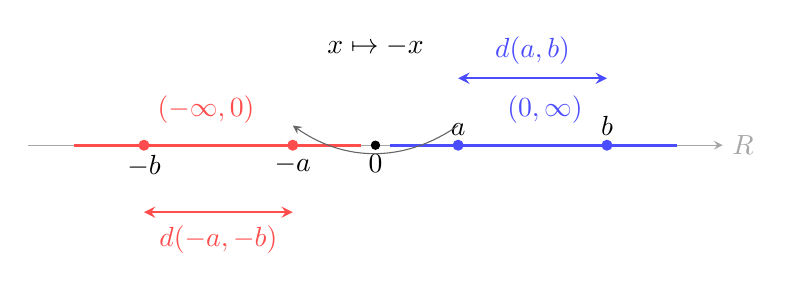
\begin{tikzpicture}[x=1.05cm,y=1cm,>=stealth]
  \draw[->,gray!70] (-4.2,0) -- (4.2,0) node[right] {\(\mathbb{R}\)};
  \fill[black] (0,0) circle (1.7pt);
  \node[below] at (0,0) {\(0\)};

  \draw[blue!70,very thick] (0.18,0) -- (3.65,0);
  \draw[red!70,very thick] (-3.65,0) -- (-0.18,0);
  \node[blue!70] at (2.05,0.45) {\((0,\infty)\)};
  \node[red!70] at (-2.05,0.45) {\((-\infty,0)\)};

  \foreach \x/\lab in {1/a,2.8/b}
  {
    \fill[blue!70] (\x,0) circle (2pt);
    \node[above] at (\x,0) {\(\lab\)};
    \fill[red!70] (-\x,0) circle (2pt);
    \node[below] at (-\x,0) {\(-\lab\)};
  }

  \draw[<->,blue!70,thick] (1,0.85) -- (2.8,0.85);
  \node[blue!70] at (1.9,1.2) {\(d(a,b)\)};
  \draw[<->,red!70,thick] (-2.8,-0.85) -- (-1,-0.85);
  \node[red!70] at (-1.9,-1.2) {\(d(-a,-b)\)};

  \draw[->,black!60] (1,0.25) to[bend left=35] (-1,0.25);
  \node at (0,1.25) {\(x\mapsto -x\)};
\end{tikzpicture}
